
\subsection{Design overview : Assumptions}

\begin{itemize}
\item It must constantly monitor
itself and detect, tolerate, and \textbf{recover promptly from
component failures on a routine basis}.
\item The system stores a modest number of large files. We
expect a few million files, each typically 100 MB or
larger in size. Multi-GB files are the common case
and should be managed efficiently. \textbf{Small files must be
supported, but we need not optimize for them.}
\item The workloads primarily consist of two kinds of reads:
\textbf{large streaming reads and small random reads}. In
large streaming reads, individual operations typically
read hundreds of KBs, more commonly 1 MB or more.
Successive operations from the same client often read
through a contiguous region of a file. A small random
read typically reads a few KBs at some arbitrary
offset. Performance-conscious applications often batch
and sort their small reads to advance steadily through
the file rather than go backand forth.
\item The workloads also have many large, sequential writes
that append data to files. Typical operation sizes are
similar to those for reads. Once written, files are seldom
modified again. \textbf{Small writes at arbitrary positions
in a file are supported but do not have to be
efficient.}
\item The system must efficiently implement well-defined semantics
for multiple clients that concurrently append
to the same file. Our files are often used as producerconsumer
queues or for many-way merging. \textbf{Hundreds
of producers, running one per machine, will concurrently
append to a file}. Atomicity with minimal synchronization
overhead is essential. The file may be
read later, or a consumer may be reading through the
file simultaneously.
\item \textbf{High sustained bandwidth is more important than low
latency}. Most of our target applications place a premium
on processing data in bulkat a high rate, while
few have stringent response time requirements for an
individual read or write
\end{itemize}

We support the usual operations to \textbf{create, delete,
open, close, read, and write files}.
Moreover, GFS has \textbf{snapshot and record append operations}.
Snapshot creates a copy of a file or a directory tree
at low cost. Record append allows multiple clients to \textbf{append
data to the same file concurrently while guaranteeing
the atomicity of each individual client’s append}.

\subsection{Architecture}

A GFS cluster consists of a single master and multiple
chunkservers and is accessed by multiple clients.

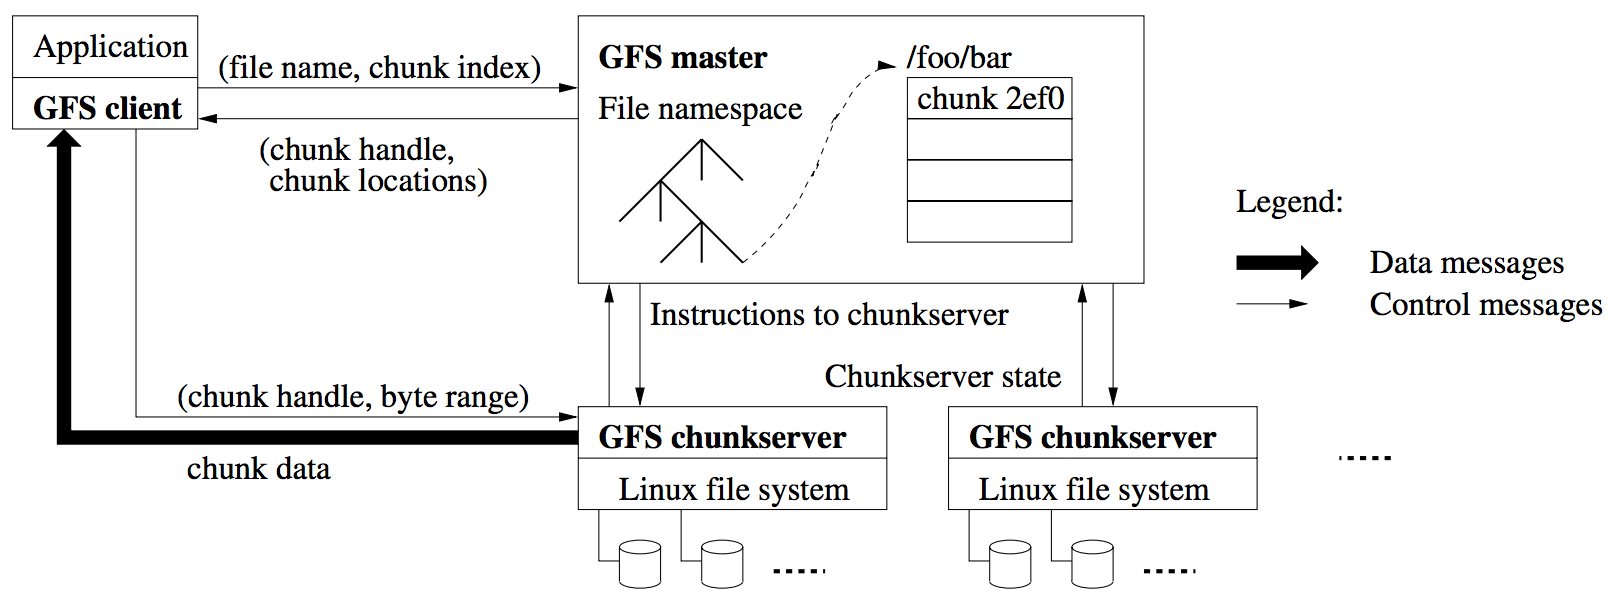
\includegraphics[width=\linewidth]{img/gfs.png}

Files are divided into fixed-size chunks. Each chunkis
identified by an immutable and globally unique 64 bit chunk
handle assigned by the master at the time of chunkcreation.
Chunkservers store chunks on local disks as Linux files and
read or write chunkdata specified by a chunkhandle and
byte range. For reliability, each chunkis replicated on multiple
chunkservers. By default, we store three replicas, though
users can designate different replication levels for different
regions of the file namespace.

The master maintains all file system metadata. This includes
the namespace, access control information, the mapping
from files to chunks, and the current locations of chunks.
It also controls system-wide activities such as chunklease
management, garbage collection of orphaned chunks, and
chunkmigration between chunkservers. The master periodically
communicates with each chunkserver in HeartBeat
messages to give it instructions and collect its state.

Clients interact with the master for metadata operations,
but all data-bearing communication goes directly to
the chunkservers.

Neither the client nor the chunkserver caches file data.
Client caches offer little benefit because most applications
stream through huge files or have working sets too large
to be cached. Not having them simplifies the client and
the overall system by eliminating cache coherence issues.
(Clients do cache metadata, however.) Chunkservers need
not cache file data because chunks are stored as local files
and so Linux’s buffer cache already keeps frequently accessed
data in memory.


\subsection{Single master}

The client typically asks for multiple chunks in the
same request and the master can also include the information
for chunks immediately following those requested. This
extra information sidesteps several future client-master interactions
at practically no extra cost. The client uses a cache for these metadata. 

\subsection{Chunk Size}

Chunksize is one of the key design parameters. We have
chosen 64 MB, which is much larger than typical file system
blocksizes. Each chunkreplica is stored as a plain
Linux file on a chunkserver and is extended only as needed.
Lazy space allocation avoids wasting space due to internal
fragmentation, perhaps the greatest objection against such
a large chunksize.

A large chunksize offers several important advantages.
First, it reduces clients’ need to interact with the master
because reads and writes on the same chunkrequire only
one initial request to the master for chunklocation information.
The reduction is especially significant for our workloads
because applications mostly read and write large files
sequentially. Even for small random reads, the client can
comfortably cache all the chunklocation information for a
multi-TB working set. Second, since on a large chunk, a
client is more likely to perform many operations on a given
chunk, it can reduce network overhead by keeping a persistent
TCP connection to the chunkserver over an extended
period of time. Third, it reduces the size of the metadata
stored on the master. This allows us to keep the metadata
in memory.

\textbf{A large chunksize, even with lazy space
allocation, has its disadvantages}.  A small file consists of a
small number of chunks, \textbf{perhaps just one}. The chunkservers
storing those chunks may become \textbf{hot spots if many clients
are accessing the same file}. In practice, hot spots have not
been a major issue because our applications mostly read
large multi-chunkfiles sequentially.

Hot spots did develop when GFS was first used
by a batch-queue system: \textbf{an executable was written to GFS
as a single-chunkfile and then started on hundreds of machines
at the same time}. The few chunkservers storing this
executable were overloaded by hundreds of simultaneous requests.
We fixed this problem by storing such executables
with a higher replication factor and by making the batchqueue
system stagger application start times. A potential
long-term solution is to allow clients to read data from other
clients in such situations.

\subsection{Metadata}

Three major types of metadata:
\begin{description}
\item[the file and chunknamespaces]
\item[the mapping from files to chunks]
\item[the locations of each chunk’s replicas] The master does not store chunklocation information persistently. Instead, it asks each chunkserver about its chunks at master startup and whenever a chunkserver joins the cluster.
\end{description}

The first two types (namespaces
and file-to-chunkmapping) are also kept persistent by
logging mutations to an operation log stored on the master’s
local diskand replicated on remote machines. Using
a log allows us to update the master state simply, reliably,
and without risking inconsistencies in the event of a master
crash.

\subsubsection{In-Memory Data Structures}

Since metadata is stored in memory, master operations are
fast. Furthermore, it is easy and efficient for the master to
periodically scan through its entire state in the background.
This periodic scanning is used to implement chunkgarbage
collection, re-replication in the presence of chunkserver failures,
and chunkmigration to balance load and diskspace usage across chunkservers.

One potential concern for this memory-only approach is
that the number of chunks and hence the capacity of the
whole system is limited by how much memory the master
has.  The cost of adding extra memory to the master is a small price to pay
for the simplicity, reliability, performance, and flexibility we
gain by storing the metadata in memory.

\subsubsection{Chunk Locations}

\textbf{The master does not keep a persistent record of which
chunkservers have a replica of a given chunk. It simply polls
chunkservers for that information at startup}. The master
can keep itself up-to-date thereafter because it controls all
chunkplacement and monitors chunkserver status with regular
HeartBeat messages.

\subsubsection{Operation Log}

The operation log contains a historical record of critical
metadata changes.

Files and chunks, as well as their versions are all uniquely and eternally identified by the logical times at which they were created.

Since the operation log is critical, \textbf{we must store it reliably
and not make changes visible to clients until metadata
changes are made persistent}. Otherwise, we effectively lose
the whole file system or recent client operations even if the
chunks themselves survive. Therefore, we replicate it on
multiple remote machines and respond to a client operation
only after flushing the corresponding log record to disk
both locally and remotely. The master batches several log
records together before flushing thereby reducing the impact
of flushing and replication on overall system throughput.

The master recovers its file system state by replaying the
operation log. To minimize startup time, we must keep the
log small.  GFS uses checkpoints to do so. The new checkpoint
includes all mutations before the switch. It can be created
in a minute or so for a cluster with a few million files. When
completed, it is written to diskboth locally and remotely.

\subsection{Consistency Model}

File namespace mutations (e.g., file creation) are atomic.
They are handled exclusively by the master: namespace
locking guarantees atomicity and correctness. The master’s operation log defines a global total order of these operations.

\textbf{A file region is consistent if all clients will
always see the same data, regardless of which replicas they
read from}. A region is defined after a file data mutation if it
is consistent and clients will see what the mutation writes in
its entirety. When a mutation succeeds without interference
from concurrent writers, the affected region is defined (and
by implication consistent): all clients will always see what
the mutation has written. \textbf{Concurrent successful mutations
leave the region undefined but consistent: all clients see the
same data, but it may not reflect what any one mutation
has written}.

Data mutations may be \textbf{writes} or \textbf{record appends}. \textbf{A write
causes data to be written at an \underline{application-specified file
offset}}. \textbf{A record append causes data (the “record”) to be
appended atomically at least once even in the presence of
concurrent mutations, but at \underline{an offset of GFS’s choosing}}. The offset is returned to the client and marks
the beginning of a defined region that contains the record.
In addition, GFS may insert padding or record duplicates in
between. They occupy regions considered to be inconsistent
and are typically dwarfed by the amount of user data.

\begin{figure}[!h]
\centering
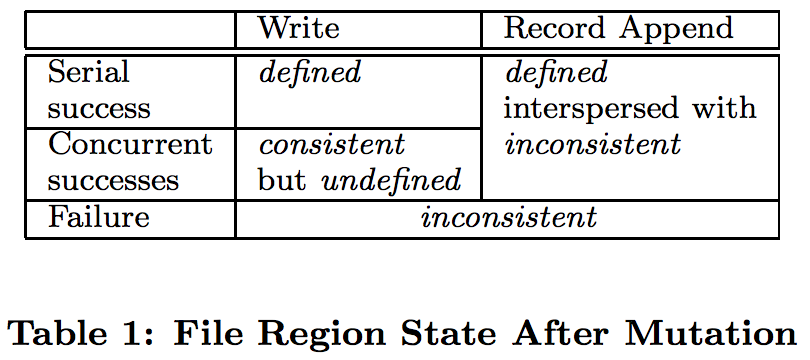
\includegraphics[width=0.6\linewidth]{img/summary_consistency_gfs.png}
\end{figure}

After a sequence of successful mutations, the mutated file
region is guaranteed to be defined and contain the data written
by the last mutation. GFS achieves this by
\begin{itemize}
\item applying
mutations to a chunkin the same order on all its replicas
\item using chunkversion numbers to detect
any replica that has become stale because it has missed mutations
while its chunkserver was down
\end{itemize}

Stale replicas will never be involved in a mutation or given to
clients asking the master for chunk locations. They are
garbage collected at the earliest opportunity.

Since clients cache chunklocations, they may read from a
stale replica before that information is refreshed. This window
is limited by the cache entry’s timeout and the next
open of the file, which purges from the cache all chunkinformation
for that file. Moreover, as most of our files are
append-only, a stale replica usually returns a premature
end of chunkrather than outdated data. When a reader
retries and contacts the master, it will immediately get current
chunklocations.

Long after a successful mutation, component failures can
of course still corrupt or destroy data. GFS identifies failed
chunkservers by regular handshakes between master and all
chunkservers and \textbf{detects data corruption by checksumming}.

A chunk is lost irreversibly only if all its replicas are lost before GFS
can react, typically within minutes. Even in this case, it becomes
unavailable, not corrupted: applications receive clear
errors rather than corrupt data.

\subsubsection{Implications for Applications}

GFS applications can accommodate the relaxed consistency
model with a few simple techniques already needed for
other purposes: relying on appends rather than overwrites,
checkpointing, and writing self-validating, self-identifying
records.

Practically all our applications \textbf{mutate files by appending
rather than overwriting}.

In the other typical use, many writers concurrently append
to a file for merged results or as a producer-consumer
queue. Record append’s append-at-least-once semantics preserves
each writer’s output. Readers deal with the occasional
padding and duplicates as follows. \textbf{Each record prepared
by the writer contains extra information like \underline{checksums}
so that its validity can be verified. A reader can
identify and discard extra padding and record fragments
using the checksums}. If it cannot tolerate the occasional
duplicates (e.g., if they would trigger non-idempotent operations),
\textbf{it can \underline{filter them out} using unique identifiers in
the records, which are often needed anyway to name corresponding
application entities such as web documents}. These
functionalities for record I/O (except duplicate removal) are
in library code shared by our applications and applicable to
other file interface implementations at Google. With that,
the same sequence of records, plus rare duplicates, is always
delivered to the record reader.

\subsection{Leases and Mutation Order}

We use leases to \textbf{maintain a consistent mutation order across
replicas}. The master grants a chunklease to one of the replicas,
which we call the primary. The primary picks a serial
order for all mutations to the chunk. All replicas follow this
order when applying mutations. Thus, the global mutation
order is defined first by the lease grant order chosen by the
master, and within a lease by the serial numbers assigned
by the primary.

The lease mechanism is designed to minimize management
overhead at the master. A lease has an initial timeout
of 60 seconds. However, as long as the chunkis being mutated,
the primary can request and typically receive extensions
from the master indefinitely. These extension requests
and grants are piggybacked on the HeartBeat messages regularly
exchanged between the master and all chunkservers.
The master may sometimes try to revoke a lease before it
expires (e.g., when the master wants to disable mutations
on a file that is being renamed). Even if the master loses
communication with a primary, it can safely grant a new
lease to another replica after the old lease expires.

\begin{figure}[!h]
\centering
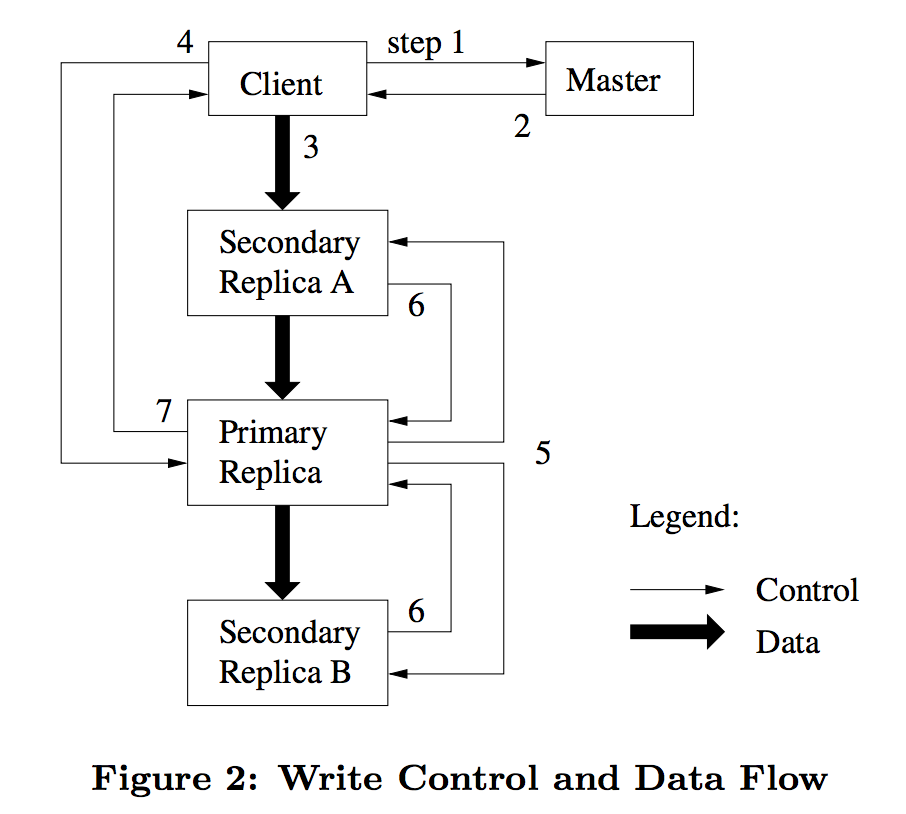
\includegraphics[width=0.6\linewidth]{img/gfs_data_control.png}
\end{figure}

Once a chunkserver receives some data, it starts forwarding immediately.
Control and data flows are decoupled.

\subsection{Snapshot}

we use standard copy-on-write techniques to
implement snapshots. When the master receives a snapshot
request, it first revokes any outstanding leases on the chunks
in the files it is about to snapshot. This ensures that any
subsequent writes to these chunks will require an interaction
with the master to find the lease holder. This will give the
master an opportunity to create a new copy of the chunk
first.

By creating the new chunkon the same chunkservers as the original, we
ensure that the data can be copied locally, not over the network(our
disks are about three times as fast as our 100 Mb
Ethernet links).


